\documentclass[conference]{IEEEtran}
% \IEEEoverridecommandlockouts
% The preceding line is only needed to identify funding in the first footnote. If that is unneeded, please comment it out.
%Template version as of 6/27/2024

\usepackage{cite}
\usepackage{amsmath,amssymb,amsfonts}
\usepackage{algorithmic}
\usepackage{graphicx}
\usepackage{textcomp}
\usepackage{xcolor}
\usepackage[]{svg}
\def\BibTeX{{\rm B\kern-.05em{\sc i\kern-.025em b}\kern-.08em
    T\kern-.1667em\lower.7ex\hbox{E}\kern-.125emX}}
\begin{document}

\title{ECE 545 Progress Report 3}

\author{\IEEEauthorblockN{Skylar Coelho}
	\IEEEauthorblockA{\textit{Electrical and Computer Engineering} \\
		\textit{University of Illinois Chicago}\\
		Chicago, USA \\
		scoelh4@UIC.edu}
}

\maketitle

\begin{abstract}
Between progress report 2 and progress report 3, I focused on finalizing the simulink model for the converter, deriving the equivalent model, deriving the gain equation, and generating test data for the machine learning model.

\end{abstract}

\section{Converter Operation}

This project utilizes a full-bridge series resonant LLC converter with synchronous rectification.
The converter topology was chosen due to its ability to achieve soft switching under both switch turn on and switch turn off.
The converter can be seen below in figure \ref{fig:llcsr}

\begin{figure}[h]
	\centering
	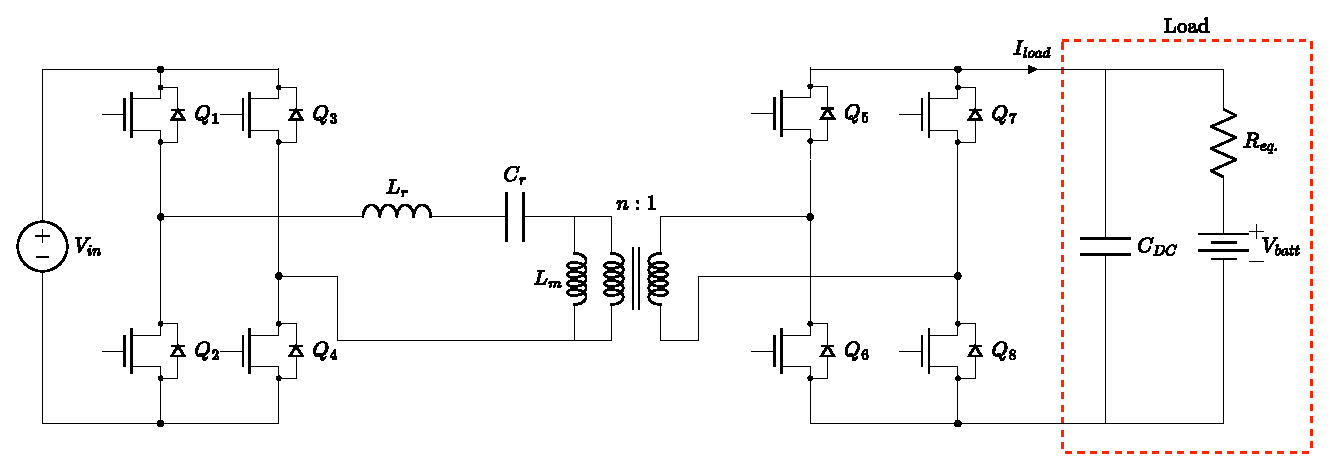
\includegraphics[width=0.7\linewidth]{figures/LLCSR}
	\caption{The full-bridge LLC series resonant converter with synchronous rectifier}
	\label{fig:llcsr}
\end{figure}



\subsection{Switching Modes}


\section{Resonant Modes}


\subsection{Resonant Mode 1}

\subsection{Resonant Mode 2}

\subsection{Resonant Mode 3}

\subsection{Resonant Mode 4}

\section{Equivalenced Circuits}

\section{Gain Derivation}

%\begin{thebibliography}{00}
%
%\end{thebibliography}

\end{document}
